\startchapter{Penalty Convex-Concave Procedure for Source Localization}% Problem}
\label{chapter:pccp}


%\section{Notes TODO}
%
%Min number of iterations: 3 - proof?
%
%stop when $\vartriangle F_{objective funstion}$ is increasing?
%
%set Max number of iterations?
%
%study the geometry of not-so-well results
%
%add cases with 5 - 15 sensors
%
%use SMACOF paper as an example of the divergence proof
%
%\phantom{m}


In connection with the problem of localizing a single radiating source based on range measurements, in this chapter we explore special structure of the cost function of an unconstrained least squares (LS) formulation and show that it is well suited in a setting known as difference-of-convex-functions (DC) programming. In the literature, the DC programming is sometimes referred to as convex-concave procedure. Our focus in this chapter will be placed on the localization problem based on range measurements. We present an algorithm for solving the LS problem at hand based on a penalty convex-concave procedure (PCCP) \cite{LBoyd} that accommodates infeasible initial points in solving a fairly large class of \textit{nonconvex} constrained problems. Algorithmic details are provided to show that the PCCP-based formulation is tailored to the localization problem at hand. These include additional constraints that enforce the algorithms iteration path towards the LS solution, and several strategies to secure good initial points. Numerical results are presented to demonstrate that the proposed algorithm
offers substantial performance improvement relative to some best known results from the literature.


%\section{Source Localization From Range Measurements}%II
\section{Problem Statement and Review of Related\\ Work}%2.1


Typically non-survey based localization techniques compute the location estimates in two steps: range/angle estimation and tri-lateration/angulation \cite{GeoLoc}. In general, the range estimates can be based on different types of measurements, e.g. received signal strength (RSS), %angle of arrival (AOA), time difference of arrival (TDOA) 
or time of arrival (TOA). %radio frequency (RF) , ultrasonic, sonic, light \cite{new book}. 
This chapter will focus on the  problem of range-based localization given the TOA information. In the TOA method, the one-way propagation time of the signal traveling between radiating source and the sensor node is measured. Each TOA measurement then provides a circle centered at the sensor node on which the source of the signal must lie. With three or more sensor nodes the measurements are converted into a set of circular equations that, with knowledge of the geometry of the sensor network, allow to determine the unknown source position \cite{GeoLoc}. The accuracy of the positioning depends on the quality of the range measurements, network geometry, and the performace of the localization algorithm. In real-world situations, multipath and non line-of-sight (NLOS) propagation are two major sources of error, which can introduce large biases in the TOA measurements and result in unreliable position esitmation \cite{classMDS}. In fact, mitigation of the impairments due to multipath and/or NLOS is another key
research topic in wireless location and recent works in this area have reported some promising results \cite{DarWinUWB}. Ultra-wideband (UWB) technology has the potential to deliver very accurate range measurements, thus enabling accurate positioning \cite{RydstromUWB, UWB, DarWinUWB}. As a result, we assume that the multipath and NLOS errors in the TOA measurements have been successfully mitigated.  

The source localization problem discussed in this chapter involves a given array of $m$ sensors placed in the $n = 2$ or 3 dimentional space with coordinates specified by $\{\Ba_1,\ldots, \Ba_m, \Ba_i\in R^n\}$. Each sensor measures its distance to a radiating source $\Bx\in R^n$. Throughout it is assumed that only noisy copies of the distance data are available, hence the \textit{range measurements} obey the model
\begin{equation} \label{eq:4.1}
\setcounter{equation}{1}
r_i = \|{\Bx} - {\Ba}_i\| + \varepsilon_i, \quad i = 1, \ldots , m.
\end{equation}    
where $\varepsilon_i$ denotes the unknown noise that has occurred when the $i$th sensor measures its distance to source $\Bx$. Let $\Br=[r_1 \ r_2 \ldots r_m]^T$ and $\Beps=[\varepsilon_1 \ \varepsilon_2 \ldots \varepsilon_m]^T$.  The source localization problem can be stated as to estimate the exact source location $\Bx$ from noisy range measurements $\Br$. 

The nonlinear least squares (NLLS) estimate refers to the solution of the problem
\begin{equation}\label{eq:4.2} %eq 2
\Min_{\Bx} \quad F(\Bx)=\sum_{i=1}^{m} (r_i - \|{\Bx} - {\Ba}_i\|)^2
\end{equation}
If ranging errors $\varepsilon_i$ are i.i.d. random variables that follow Gaussian distribution with zero mean and covariance matrix proportional to the identity matrix, then the NLLS estimate becomes identical to the maximum likelihood estimate. The NLLS formulation is also geometrically meaningful and has been often used as a benchmark to compare new algorithms \cite{BeckStLi,UWB}. 

%re-phrase the below
%\textit{
%Non linear least squares  \cite{UWB, GhStr}, (check ref) provide an accurate solution / generally perform well \cite{UWB, GhStr}. and .... NLLS has often been used as a benchmark to compare more novel algorithms \cite{UWB, BeckStLi, more-more}....
%Moreover, in some cases ( mention that review paper from 2010) the PDF may not be available. In some literature the NLLS \textit{cite GhStr} was mentioned to perform well for range measurements if it the solution converged to the global minimum.
%}


In Sec.2.1 of the thesis, it is demonstrated that these problems are hard to solve globally. Many relaxation and approximation methods were developed that offer either lower computational complexity, robustness against positive bias in the distance estimates due to non line-of-site situations, or better performance compared to standard unconstrain optimization methods applied to the NLLS problem. Convex relaxation of a nonconvex problem in (\ref{eq:4.2}) to an SDP problem and solution methods for \textit{squared} range LS problems are discussed in detail in \cite{IRWSg} and  Sec.2.1 and of the thesis. Another localization approach that has received considerable interest applies classical multidimensional scaling (MDS) algorithm or its variants to the problem at hand \cite{classMDS, fastMDS, dwMDS, genMDS}. 

%\textbf{
%Multidimensional scaling (MDS) algorithm is an attractive technique for analysing experimental data in psychology, geography and molecular biology and is also used to determine the relative coordinates of points given only their pairwise distances.
Multidimensional scaling is a field of study concerning the search of points in a
low dimensional space that represent the objects of interest and the pairwise distances between the points (objects) (as measure of dissimilarities) match a set of given values. As such MDS has been an attractive technique for analyzing experimental data in physical, biological, and behavioral science  \cite{classMDS}. The classical MDS is a subset of MDS techniques where the relative coordinates of points  are determined given only their pairwise Euclidean distances.
%By the same principle, it is expected that the MS location can be determined if the distances among the MS and BSs are provided.
%
%Classical MDS was first introduced in the discipline of psychology and its basic idea is to assume that the dissimilarities between objects are distances and then find coordinates that explain them.
%
%MDS provides fast and globally convergence solution
%}

%The main assumptions about this procedure are: sensor nodes are able to obtain pairwise distances between and these measurements are free of noise; range measurement errors between the sensors and source $\Bx$ are i.i.d. Gaussian variables with zero mean and \textit{known} variance. In brief the MDS algorithm can be described as follows

When applied to the localization problem at hand, classical MDS starts with constructing a multidimentional similarity matrix. Let $\BX$ denote  an $m$ x $n$ distance matrix 
\begin{equation}
\nonumber
\begin{aligned}
\BX = \left( \begin{array}{c}
(\Bx - \Ba_1)^T \\
(\Bx - \Ba_2)^T \\
\vdots \\
(\Bx - \Ba_m)^T
\end{array}
\right) 
\\
\end{aligned}
\end{equation}
The multidimentional similarity matrix is then defined by $\BD = \BX\BX^T$ which can also be expressed in terms of pairwise distances between sensor nodes and error-free range measurements. Since the exact distances between the sourse $\Bx$ and sensors are not available, the noisy range measurements $r_i$ are used to construct an approximation of $\BD$ as %approximate version of $\BD$, denoted $\hat{\BD}$ as
\begin{equation}
\nonumber
\hat{\BD}\!=\!\frac{1}{2}\!\left(\!\!\begin{array}{cccc}
2r_1^2 & r_1^2 + r_2^2 - \|\Ba_1 - \Ba_2\|^2 & \ldots & r_1^2 + r_m^2 - \|\Ba_1 - \Ba_m\|^2\\
r_1^2 + r_2^2 - \|\Ba_1 - \Ba_2\|^2 & 2 r_2^2 & \ldots & r_2^2 + r_m^2 - \|\Ba_2 - \Ba_m\|^2\\
\vdots & \vdots & \ddots & \vdots \\
r_1^2 + r_m^2 - \|\Ba_1 - \Ba_m\|^2 & r_2^2 + r_m^2 - \|\Ba_1 - \Ba_m\|^2 & \ldots & 2r_m^2\end{array}\!\right) \\
\end{equation}
%Since $\hat{\BD}$ is symmetric and positive semi-definite, it can be decomposed  using eigenvalue factorization
Because matrix $\hat{\BD}$ is symmetric, it admits the orthogonal eigen-decomposition
\begin{equation}
\nonumber
\hat{\BD} = \BU\BLA\BU^T
\end{equation}
where $\BLA = \mbox{diag}\left(\lambda_1, \lambda_2, \ldots, \lambda_m\right)$ is the diagonal matrix of eigenvalues of $\hat{\BD}$ with $\lambda_1 \geq \lambda_2 \geq \ldots \geq \lambda_m \geq 0$, and $\BU = \left[\Bu_1 \quad \Bu_2  \ldots \Bu_m \right]$ is an orthonormatl matrix whose columns are the corresponding eigenvectors. Since the rank of the ideal $\BD$ is 2, an LS estimate of $\BX$, denoted by $\BX_r$, can be computed up to an arbitrary rotation as a solution to the following problem  \cite{classMDS}
\begin{equation}
\nonumber
\BX_r = \mbox{arg}\min_{\tilde{\BX}} \|\hat{\BD} - \tilde{\BX}\tilde{\BX}^T\|^2_{F} = \BU_s\BLA_s^{(1/2)}
\end{equation}
where $\tilde{\BX}$ is the variable matrix for $\BX$, $\|.\|_F$ represents the Frobenius norm, $\BU_s = \left[\Bu_1 \ \ \Bu_2\right]$ corresponds to the signal subspase, and $\BLA^{(1/2)} = \mbox{diag}(\lambda_1^{(1/2)}, \lambda_2^{(1/2})$. In practical situations of nonzero range errors, the relationship between  $\BX_r$ and $\BX$ is then 
\begin{equation}
\nonumber
\BX  \approx \BX_r\BOmega
\end{equation} 
where $\BOmega$ is an unknown rotation matrix to be determined. The estimate of the unknown rotation matrix $\BOmega$ and source location $\Bx$ can be obtained by solving an overdetermined system of linear equations \cite{classMDS}. In the absence of noise the symmetric $\hat{\BD}$ is identical to $\BD$, is positive semi-definite, and has a rank of 2. In the practical situations of nonzero range errors, $\hat{\BD}$ will have a full rank. 

Other methods based on MDS include a generalized subspace approach by So and Chan \cite{genMDS}, that performs  position estimation based on the noise subspace. A subspase-based weighting Lagrangian multiplier estimator \cite{fastMDS} reduces computational complexity by avoiding the process of eigendecomposition or inverse computation, but it requires some a priori knowledge about noise statistic to construct the weighting matrix. On the other hand, the distributed weighted-multidimentional scaling (DW-MDS) \cite{dwMDS} adds a penalty term to the standard MDS objective function which accounts for prior knowledge about node locations. Although these methods work well in general and can be efficient in terms of complexity, they
are found to produce poor performance in certain sensor deployments  \cite{UWB}.

%Although these methods can be efficient in terms of complexity and generraly work well, they can show poor performance in certain sensor deployments \cite{UWB}.%they remain to be suboptimal in the maximum likelihood (ML) sence.

%\textit{It is assumed that range measurement errors between the sensors and source $\Bx$ are i.i.d. Gaussian variables with zero mean and \textit{known} variance. }
%Gheung and So \cite{classMDS} proposed a range-based localization algorithm based on a modified classical MDS. The main assumptions about this procedure are: sensor nodes are able to obtain pairwise distances between and these measurements are free of noise; range measurement errors between the sensors and source $\Bx$ are i.i.d. Gaussian variables with zero mean and \textit{known} variance. In brief the MDS algorithm can be described as follows

 
In this chapter, we focus on the least squares formulation for the localization problem, where the $l_2$-norm of the residual errors is minimized in a setting known as difference-of-convex-functions programming. The problem at hand is then solved by applying a penalty convex-concave procedure (PCCP) in a succesive manner \cite{PCCP}.

%%%%%%%%% comment start
%Locating a radiating source from range measurements in a passive sensor network has recently attracted an increasing amount of research interest as it finds applications in a wide range of network-based wireless systems. Least squares (LS) based algorithms for source localization problems constitute an important class of solution techniques as they are geometrically meaningful and often provide low complexity solution procedures with competitive  estimation accuracy \cite{Chan}-\cite{BeckStLi}.  On the other hand, the error measure in an LS formulation for the localization problem of interest is shown to be highly non-convex, possessing multiple local solutions with degraded performance. This non-convexity excludes many local methods that are iterative, hence extremely sensitive to where the iteration begins. Several non-iterative \textit{global}  localization techniques are available from the literature. 
%% In the case of source localization, this inherent feature of local methods is particular problematic because the source location is assumed to be entirely unknown and can appear practically anywhere. 
%%, thus the chances to secure a good initial point for a local algorithm are next to none. For these reasons, we are interested in \textit{global} localization techniques that are either non-iterative or insensitive to initial iterate. 
%A global solution may be obtained by relaxing the LS model at hand to a semidefinite programming (SDP) problem which is known to be convex \cite{VBoyd}. In doing so, however, the convexification based solution is no longer optimal in LS sense. Another representative in this class is the method proposed in \cite{BeckStLi}, where localization problems for  range measurements are addressed by developing solution methods for \textit{squared} range LS (SR-LS) problems. Although these methods are efficient in terms of complexity, they remain to be suboptimal in the maximum likelihood (ML) sense because the solutions produced are merely approximations of the ML estimate.

%%%%%%%%% comment end

%One representative in the class of global localization methods is the convex-relaxation based algorithm proposed in \cite{Cheung}, where the LS model is relaxed to a semidefinite programming (SDP) problem which is known to be convex \cite{VBoyd}. 
%%\textit{``However, as discussed in [3], the optimal solution of this relaxed SDP does not always satisfy the near-rank-1 constraints of acceptable solutions to the source localization problem.''} 

% However, the solution provided by these algorithms is less accurate than than those produced by ML approaches, \textit{`'because they are suboptimal in the ML sence.''}
%In this  paper we minimize the $l_2$ norm of residual errors and present it as a differece of convex functions programming (DCP). 
%In this paper we exploit the special structure of the cost function of an unconstrained LS formulation for the localization problem. In particular we present it as a difference of convex functions (DC) programming problem and  solve it by applying a constrained convex-concave procedure (CCCP), which is an effective heuristic method to deal with this class of problems \cite{Yu,LBoyd}. 
%\textit{``Lu-Hinamoto: We show that a constrained optimization setting known as convex-concave procedure \cite{Huang,Cheung}, when applied in a successive manner, is naturally suited for the design of stable composite filters where the FIR and IIR components are jointly optimized in frequency-weighted minimax sense.''} 
% A penalty CCCP \cite{LBoyd} allows to extend the algorithm to accept infeasible initial points by introducing additional slack variables, which is highly important for the case of a non-convex localization problem at hand for which a feasible initial point is hard to secure.
% \textit{`` By introducing additinoal slack variables, a penalty CCP has been developed to accept infeasible initial points''}. 
% We further extend the flexibility of the approach by proposing the  method of choosing the initial point for the algorithm.   Numerical results show that the proposed approach can offer substantial performance improvement relative to the existing suboptimal estimators.
% We focus on the LS formulation since it is known to be the maximum-likelihood estimator in the case of Gaussian white measurement noise and therefore would provide most accurate solution. Numerical results are presented for performance evaluation and comparisons.

%for which a variation of the convex-concave procedure (CCP) has been proposed  in [ref], a powerful heuristic method for this type of 

%of the LS problem, which is unconstrained, and treat it as a difference of convex functions (DC) program and apply an extended version of the convex-concave procedure. The basic CCP requires a feasible initial point x0 to start the procedure. By introducing additional slack variables, a penalty CCP has been developed to accept infeasible initial points.


%The key new ingredient of the proposed algorithms is an iterative procedure where the SR-LS (or SRD-LS) algorithm is applied to a weighted sum of squared terms where the weights are carefully designed so that the iterates produced quickly converge to a solution which, on comparing with the best known results, is found to be considerably closer to the original range-based (or range-difference-based)

%\subsubsection{convex relaxation on the convex plane}

%[ASSP10] ``An approximate solution to the maximum likelihood location estimation problem is proposed, by redefining the problem in the complex plane and relaxing the minimization problem into semidefinite programming form. ... Our relaxation for source localization in the complex plane (SLCP) is motivated by the near-convexity of the objective function and constraints in the complex formulation of the original (non-relaxed) problem.''


%%%%%%%%% comment start
%Formulation (\ref{eq:4.2}) is connected to the maximum-likelihood (ML) location estimation that determines $\Bx$ by examining the probabilistic model of the error vector $\Beps$. If $\Beps$ obeys a Gaussian distribution with zero mean and covariance $\symb{\Sigma} = \mbox{diag}(\sigma_1^2, \ldots, \sigma_m^2)$, then the maximum likelihood (ML) location estimator in this case is known to be
%\begin{equation} \label{eq:4.3}%eq 3
%\Bx_{ML} = \mbox{arg}\!\min_{{\Bx} \in R^n} (\Br - \Bg)^T\Sigma^{-1}(\Br - \Bg)
%\end{equation}
%where $\Bg = [g_1 \ g_2 \ldots \ g_m]^T$ with $g_i = \|{\Bx} - {\Ba}_i\|$. It follows immediately that the ML solution in (\ref{eq:4.3}) is identical to the R-LS solution of problem (\ref{eq:4.2}) when covariance $\symb{\Sigma}$ is proportional to the identity matrix, i.e., $\sigma_1^2=\ldots =\sigma_m^2 = 1$. In the literature this is known as the equal noise power case. For notation simplicity this paper focuses on the equal noise power case, however the method developed below is also applicable to the unequal noise power case by working on a weighted version of the objective in  (\ref{eq:4.2})  with $\{\sigma_i^{-2}, i = 1, \ldots, m\}$ as the weights.
%
% There are many methods for continuous unconstrained optimization \cite{AntonLu}, however most of them are \textit{local} methods in the sense they are sensitive to the choice of initial point, and give no guarantee to yield global solutions when applied to non-convex objective functions. Unfortunately, the objective function in (\ref{eq:4.2}) is highly non-convex, possessing many local minimizers even for small-scale systems. In this paper we present an different approach to solve the positioning problem, which employs a successive convex-concave procedure.

%%%%%%%%% comment end

%Reference \cite{Cheung} addresses problem (\ref{eq:4.2}) by a convex relaxation technique where (\ref{eq:4.2}) is modified to a convex problem known as semidefinite programming \cite{VBoyd}. A rather different approach is proposed in \cite{BeckStLi} where the localization problem (\ref{eq:4.2}) is tackled by developing techniques to address the \textit{squared range based LS} (SR-LS) problem
%\begin{equation} \label{eq:4.4}%eq 4
%\Min_{\Bx} \sum_{i=1}^{m} (\|{\Bx} - {\Ba}_i\|^2 - r_i^2)^2
%\end{equation}
%whose global solution can be computed by converting (\ref{eq:4.4}) into the class of generalized trust region subproblems (GTRS) \cite{More, FortinWol} and exploring its KKT conditions which are both necessary and sufficient optimality conditions. Although SR-LS solves (\ref{eq:4.4}) exactly, the produced solution remains to be an approximation of the original LS problem in (\ref{eq:4.2}) because it is no longer a ML solution. 
%
%(in this work...)

\phantom{m}

\section{Fitting the Localization Problem into a CCP Framework}% or Penalty CCCP}

\subsection{Basic Convex-Concave Procedure}


The CCP refers to an effective heuristic method to deal with a class of difference of convex (DC) programming problems, which assume the form 
\begin{eqnarray}\label{eq:DC}%eq 5
\setcounter{abc}{1}
 \Min_{\Bx} & {} & f(\Bx) - g(\Bx)  %\nonumber 
\\ \mbox{subject to:} & {} & f_i(\Bx) \leq g_i(\Bx) \quad \mbox{for: }  i = 1, 2, \ldots, m 
 \setcounter{equation}{3}
 \stepcounter{abc}
\end{eqnarray}  
where $f(\Bx), g(\Bx), f_i(\Bx), g_i(\Bx)$ for $i = 1, 2, \ldots, m$ are convex. A DC program is not convex unless the functions $g$ and $g_i$ are affine, and therefore is hard to solve in general.  The class of DC functions is very broad. For example, any $C^2$ function can be expressed as a difference of convex functions \cite{Har}. Classes of problems that can be expressed as difference of convex programming among others include Boolean linear program, circle packing, circuit layout, and multi-matrix proncipal component analysis, examples of which can be found in \cite{LBoyd} and references therein. 

The basic CCP algorithm is an iterative procedure including two key steps (in the $k$-th iteration where iterate $\Bx_k$ is known):

(i) Convexification of the objective function and constraints by replacing $g(\Bx)$ and $g_i(\Bx)$, respectively, with their affine approximations
\begin{equation} \label{eq:i}%eq 5
\setcounter{equation}{4}
\setcounter{abc}{1}
\hat{g}(\Bx,\Bx_k)   =    g(\Bx_k) +  \bigtriangledown g(\Bx_k)^T(\Bx - \Bx_k)  %\nonumber
\end{equation}
and
\begin{eqnarray}
\begin{aligned} 
\setcounter{equation}{4}
\stepcounter{abc}
\hat{g}_i(\Bx,\Bx_k)  =   g_i(\Bx_k) +  \bigtriangledown g_i(\Bx_k)^T(\Bx - \Bx_k)   & {} \\
\hfill \  \mbox{for: }  i = 1, 2, \ldots, m &{}
\end{aligned}
\end{eqnarray}

(ii) Solving the convex problem
\begin{eqnarray} \label{eq:ii}%eq6
\setcounter{equation}{5}
\setcounter{abc}{1}
 \Min_{\Bx}  & &f(\Bx) - \hat{g}(\Bx, \Bx_k) 
\\ \mbox{subject to:} & &f_i(\Bx) -  \hat{g}_i(\Bx, \Bx_k) \leq 0  
 \setcounter{equation}{5}  
 \stepcounter{abc} \\ 
\quad & & \mbox{for: }  i = 1, 2, \ldots, m \nonumber
\end{eqnarray}
Because of the convexity of all the functions involved, it can be shown that the basic CCP is a descent algorithm and the iterates $\Bx_k$ converge to the critical point of the original problem \cite{LBoyd}. In fact, the global convergence analysis for CCP has also been studied \cite{CCPConv, CCPGlob}. Note that functions $g(\Bx)$ and $g_i(\Bx)$ for $i = 1, 2, \ldots, m$ are required to be convex but not necessarily differentiable. If any of  $g(\Bx)$ or $g_i(\Bx)$ are not differentiable at some point $\tilde{\Bx}$ then the corresponding term $\bigtriangledown g(\tilde{\Bx})$ (or $\bigtriangledown g_i(\tilde{\Bx})$) is replaced by a subgradient  of $g(\Bx)$ (or $g_i(\Bx)$) at point $\tilde{\Bx}$.

Let $\mathcal{D}$ be a nonempty set in $R^n$. A vector $\Bh \in R^n$ is said to be a subgradient of  a convex function $f:\mathcal{D} \rightarrow R$  at $\Bx \in \mathcal{D}$ if
\begin{equation}
\nonumber
f(\By) \geq f(\Bx) + \Bh^T (\By - \Bx) \mbox{ for all } \By \in \mathcal{D} \\
\end{equation}
Geometrically, the subgradients
at a point  $\Bx$ for the case where the convex function $f(x)$ is not differentiable correspond to different tangent lines at $\Bx$  \cite{AntonLu}.

% \textit{ other Advantages of convex-concave procedure from cite{LBoyd}} 
 
% \phantom{m}

\begin{figure*}%[t]
\centering
  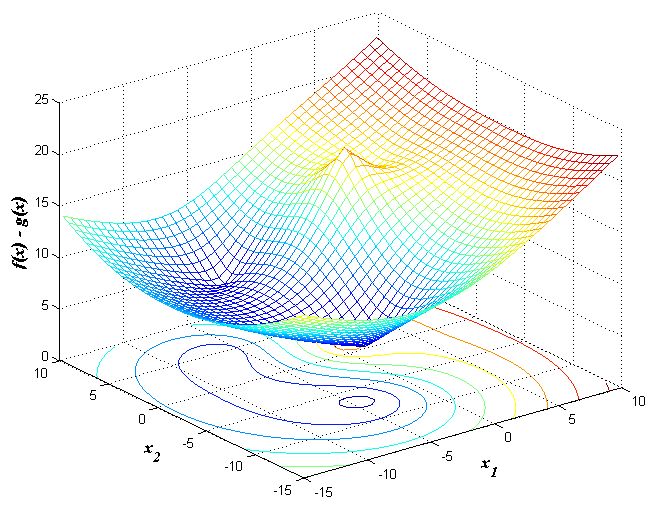
\includegraphics[width=0.85\textwidth,height=0.45\textheight]{figures/ccp/ccp_a}
   
  (a) A nonconvex function in the form of the difference of two convex functions and its contour plot.
  
  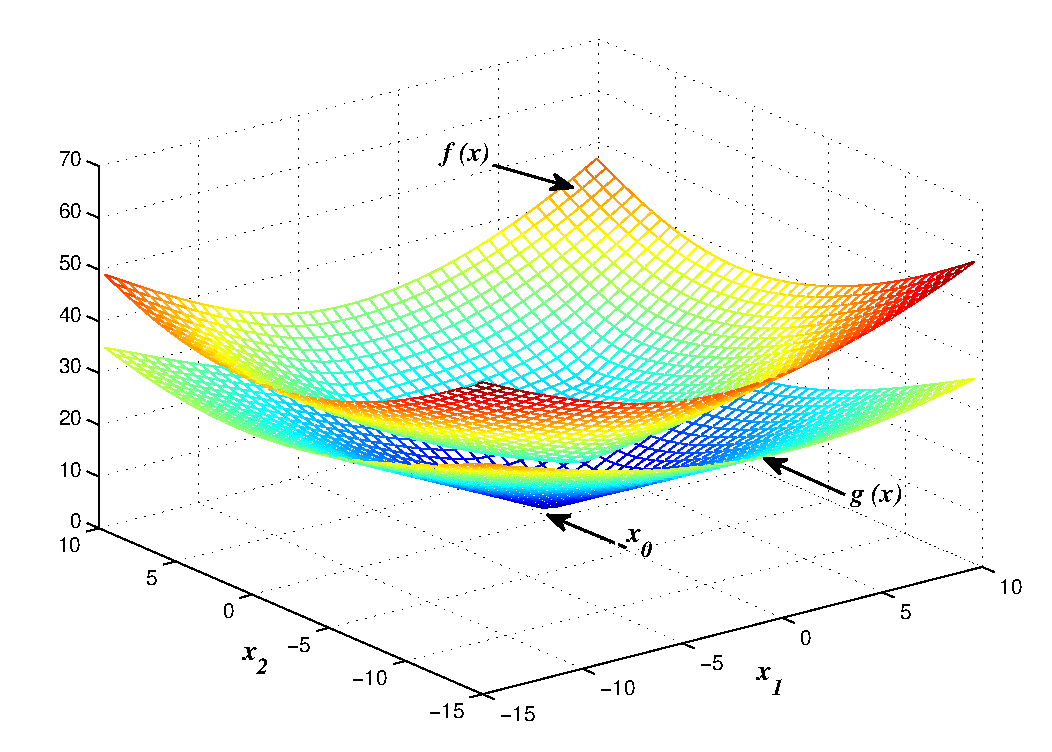
\includegraphics[width=0.9\textwidth,height=0.45\textheight]{figures/ccp/ccp_b}
  
  (b) Separation of the nonconvex function into two convex functions $f(\protect\Bx)$ and $g(\protect\Bx)$.
\end{figure*} \label{fig:ExampleCCP}
\begin{figure*}%[t]
\centering
  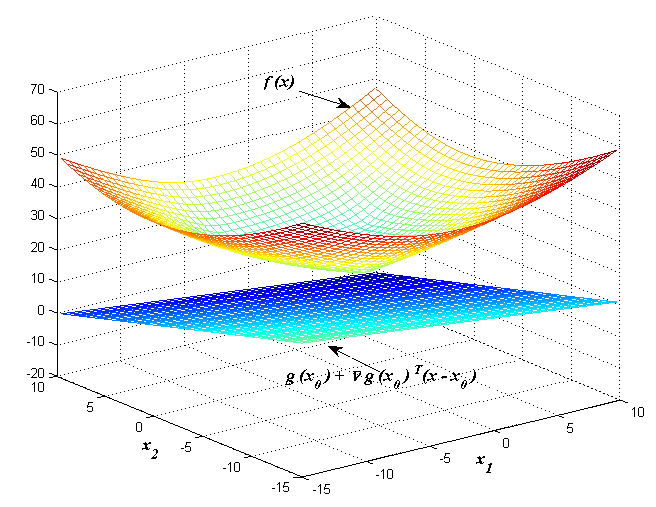
\includegraphics[width=0.85\textwidth,height=0.45\textheight]{figures/ccp/ccp_c}
  
  (c) First order approximation of $g(\protect\Bx)$.%the second function
  
  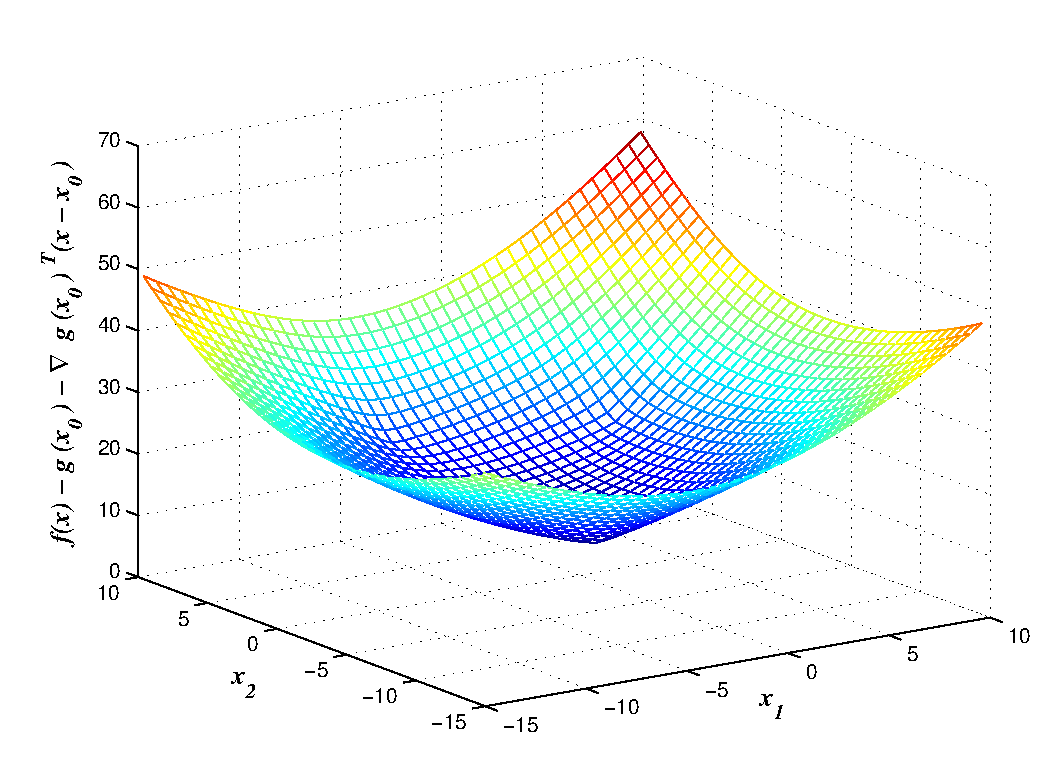
\includegraphics[width=0.85\textwidth,height=0.45\textheight]{figures/ccp/ccp_d}
  
  (d) A convex approximation of the original nonconvex function at $\protect\Bx_0$ = [0 0]$\protect^T$. 
\caption{An example of the CCP procedure (re-generated based on \cite{clock}).}
\label{fig:ExampleCCP}
\end{figure*}

Figure \ref{fig:ExampleCCP} shows an example of the CCP approach for an unconstrained DC problem in the form of (\ref{eq:DC}a), where $f(\Bx)$ and  $g(\Bx)$ are given by:
\begin{eqnarray}
\nonumber
f(\Bx) & = & \|\Bx - \Ba_1\| + \|\Bx - \Ba_2\| + \|\Bx - \Ba_3\| \\
\nonumber
g(\Bx) & = & \|2\Bx - \Ba_4\|
\end{eqnarray}
with $\Ba_1$ = [3 2]$^T$, $\Ba_2$ = [−6 5]$^T$, $\Ba_3$ = [−4 −7]$^T$, and $\Ba_4$ = [1 2]$^T$. In this figure, the original nonconvex problem is transferred to a convex problem by replacing a nonconvex part $(-g(\Bx))$ by its affine approximation around the point $\Bx_0$ = [0 0]$^T$.

\phantom{m}

\phantom{m}
 
The basic CCP requires a \textit{feasible} initial point $\Bx_0$ (in the sense that $\Bx_0$ satisfies (\ref{eq:ii}) for $ i = 1, 2, \ldots, m$)  to start the procedure. By introducing additional slack variables, a penalty CCP has been adopted to accept infeasible initial points. In what follows, we reformulate our localization problem to fit it into the basic CCP framework. Bounds on squared measurement errors as well as penalty terms are then imposed, and a PCCP-based algorithm is developed for solving the problem.

%\phantom{m}

\subsection{Problem Reformulation}

We begin by re-writing the NLLS objective function in (\ref{eq:4.2}) up to a constant as
\setcounter{abc}{0} 
\begin{equation} \label{eq:F}
%\begin{aligned}
 F(\Bx) =  m\Bx^T\Bx - 2 \Bx^T\sum^m_{i=1} \Ba_i
  - 2\sum^m_{i = 1} r_i \|\Bx - \Ba_i\| 
%\end{aligned}
\end{equation}
The objective in (\ref{eq:F}) is not convex. This is because, for points $\Bx$ that are not coincided with $\Ba_i$ for $1 \leq i \leq m$ , the Hessian of $F(\Bx)$ is given by
\begin{equation}
\nonumber
\bigtriangledown ^2 F(\Bx)  = 2m\BI  + %&
2\sum^m_{i=1} \frac{r_i}{\|\Bx - \Ba_i\|^3} \cdot %\\ \cdot &
\left( \left(\Bx - \Ba_i\right)\left(\Bx - \Ba_i\right)^T - \|\Bx - \Ba_i\|^2 \BI \right)
\end{equation}
which is obviously not always positive semidefinite.  On the other hand, by defining 
\begin{equation}  \label{eq:4.7}
\begin{aligned}
& f(\Bx) =  %\sum_m^{i = 1} \|\Bx - \Ba_i\|^2 \\
%& = m
%\Bx^T\Bx - \frac{2}{m}\Bx^T\left(\sum^m_{i=1} \Ba_i\right) \\% + \sum^m_{i=1} \|\Ba_i\|^2\\
%& g(\Bx) = \frac{2}{m}\sum^m_{i = 1} r_i \|\Bx - \Ba_i\|
m \Bx^T\Bx - 2 \Bx^T\sum^m_{i=1} \Ba_i \\% + \sum^m_{i=1} \|\Ba_i\|^2\\
& g(\Bx) = 2 \sum^m_{i = 1} r_i \|\Bx - \Ba_i\|
\end{aligned}
\end{equation}
the objective in (\ref{eq:F}) can be expressed as% difference of two convex functions 
\begin{equation}
\nonumber
F(\Bx) = f(\Bx) - g(\Bx)
\end{equation} with both $f(\Bx)$ and $g(\Bx)$ convex, hence it fits naturally into (\ref{eq:DC}). Note that $g(\Bx)$ in (\ref{eq:4.7}) is not differentiable at the point where $\Bx = \Ba_i$ for some $1 \leq i \leq m$, thus we replace the term $\bigtriangledown g(\Bx_k)$ in (\ref{eq:i}) by a subgradient \cite{Nes} of $g(\Bx)$ at $\Bx_k$, denoted by $\partial g(\Bx_k)$, as
\begin{equation} % eq:4. 9
\nonumber
\begin{aligned}
\partial g{(\Bx_k)} & = 2 \sum^m_{i = 1} r_i \partial \|\Bx_k - \Ba_i\| 
\end{aligned}
\end{equation}
where
\begin{equation}
\nonumber
\partial \|\Bx_k - \Ba_i\|  = \left\{
	\begin{aligned}
	& \frac{\Bx_k - \Ba_i}{\|\Bx_k - \Ba_i\|}, &\mbox{if } \Bx_k \neq \Ba_i \\
	& \BO, &\mbox{otherwise }%\mbox{for any } 
	\end{aligned}
\right.
\end{equation}
Hence  $\hat{g}(\Bx, \Bx_k)$ in (\ref{eq:i}) is given by
\begin{equation} % eq:4.10
\nonumber
\begin{aligned}
 \hat{g}(\Bx, \Bx_k)& =   2 \sum^m_{i=1} r_i \|\Bx_k - \Ba_i\|   +  2 \left( \Bx - \Bx_k \right)^{T} \sum^m_{i=1} r_i \partial \|\Bx_k - \Ba_i\| \\
& = 2\Bx^T \sum^m_{i=1} r_i \partial \|\Bx_k - \Ba_i \| + c
%&  =  2 \sum^m_{i=1} r_i \|\Bx_k - \Ba_i\| \\
%&+ 2\left[ \left( \Bx - \Ba_i \right) - \left( \Bx_k - \Ba_i \right)\right]^T \sum^m_{i=1} r_i \partial \|\Bx_k - \Ba_i\| \\
%& = 2 \left(\Bx - \Ba_i\right)^T \sum^m_{i=1} r_i \partial \|\Bx_k - \Ba_i\|
 \end{aligned}
\end{equation}
where $c$ is a constant given by 
\begin{equation}
\nonumber
\begin{aligned}
 c & =  2\sum^m_{i=1} r_i \|\Bx_k - \Ba_i\|   -  2 \Bx_k^T \sum^m_{i=1} r_i \partial \|\Bx_k - \Ba_i\| \\
& =  2\sum^m_{i=1} r_i \|\Bx_k - \Ba_i\|   -  2 \sum^m_{i=1} r_i \Bx_k^T \partial \|\Bx_k - \Ba_i\| \\
& = 2\sum^m_{i=1} r_i \|\Bx_k - \Ba_i\|   -  2 \sum^m_{i=1} r_i \left(\Bx_k^T - \Ba_i +\Ba_i\right)^T\partial \|\Bx_k - \Ba_i\| \\
& = 2\sum^m_{i=1} r_i \|\Bx_k - \Ba_i\|  -  2 \sum^m_{i=1} r_i \left(\Bx_k^T - \Ba_i\right)^T\partial \|\Bx_k - \Ba_i\| -2 \sum_{i = 1}^m r_i \Ba_i^T \partial \|\Bx_k - \Ba_i\| \\ 
& =  2\sum^m_{i=1} r_i \|\Bx_k - \Ba_i\| -  2\sum^m_{i=1} r_i \|\Bx_k - \Ba_i\| -2 \sum_{i = 1}^m r_i \Ba_i^T \partial \|\Bx_k - \Ba_i\| \\
& =  -2 \sum_{i = 1}^m r_i \Ba_i^T \partial \|\Bx_k - \Ba_i\|.
\end{aligned}
\end{equation}
%
%\begin{equation}
%\nonumber
%c = -2 \sum_{i = 1}^m r_i \Ba_i^T \partial \|\Bx_k - \Ba_i\|.
%\end{equation}
The convex approximation of the objective in (\ref{eq:F}) can now be derived as 
\begin{equation}
\nonumber
\begin{aligned}
\hat{F}(\Bx) & =  f(\Bx) - \hat{g}(\Bx, \Bx_k) \\
& =  m \Bx^T\Bx - 2 \Bx^T\sum^m_{i=1} \Ba_i - 2\Bx^T \sum^m_{i=1} r_i \partial \|\Bx_k - \Ba_i \| + c
\end{aligned}
\end{equation} 
It follows that, up to a multiplicative factor $1/m$ and an additive constant term, the convex objective function in (\ref{eq:ii}) can  be written as 
%Dividing by $m$ and neglecting a constant term the objective function can therefore be written as:
\begin{equation} \label{eq:4.8} 
\Min_{\Bx} \quad \hat{F}(\Bx) = \Bx^T\Bx - 2\Bx^T {\Bv}_k
\end{equation}
where
\begin{equation} \label{eq:4.9} 
\begin{aligned}
\Bv_k  = \bar{\Ba} + \frac{1}{m} \sum^m_{i=1} r_i \partial \|\Bx_k - \Ba_i\| , \quad \bar{\Ba} = \frac{1}{m}  \sum^m_{i = 1} \Ba_i 
\end{aligned}
\end{equation}
It is rather straightforward to see that given $\Bx_k$ (in the $k$-th iteration) the solution of the quadratic problem (\ref{eq:4.8}) can be obtained as
\begin{equation} \label{eq:4.10} 
\Bx_{k+1} = \bar{\Ba} + \frac{1}{m} \sum^m_{i=1} r_i \partial \|\Bx_k - \Ba_i\|.
\end{equation}
%
%The new objective $\hat{F}(\Bx)$  is convex, more particularly, quadratic, hence for any \textit{fixed} $\Bx_k$, i.e. at the $k$-th iteration, the solution of the problem (12) can be obtained as
%
%"we use the following updating formula"
%"The convex problem in (12) can now be efficiently solved. 
%Denoting the solution of (12) as $\Bx_{k+1}$, next we go for further
%improving the solution by convexifying (4) for new point $\Bx_{k+1}$
%similar to the procedure performed for $\Bx_{k}$. This sequential
%programming procedure continues for a number of iterations."
%	
\subsection{Imposing Error Bounds and Penalty Terms }

The algorithm being developed can be enhanced by imposing a bound on each squared measurement error, namely
\begin{equation} % eq:4.12
%\nonumber
\left(\|\Bx - \Ba_i\| - r_i \right)^2 \leq \delta_i^2
\end{equation}
which leads to
%\begin{equation} %eq:4.13
%\begin{aligned}
\begin{eqnarray}\label{eq:4.12}
\setcounter{abc}{1}
\|\Bx - \Ba_i\| - r_i -  \delta_i   \leq 0 \\ %\gamma \sigma_i
\stepcounter{abc}
\setcounter{equation}{12}
r_i - \delta_i \leq \|\Bx - \Ba_i\| 
%\end{aligned}
%\end{equation}
\end{eqnarray} 
for $ 1 \leq i \leq m$. 
Placing such bounds means that as iterations proceed the new iterates (coordinates of possible source locations)  are restricted to lie within a  physically meaningfull region determined by
parameters $\delta_i$.
 
Note that the constraints in (\ref{eq:4.12}a) are convex and fit into the form of basic CCP in (\ref{eq:ii}) with $f_i(\Bx) = \|\Bx - \Ba_i\| - r_i -  \delta_i $ and $g_i(\Bx) = 0$, while those in (\ref{eq:4.12}b) are in the form of (\ref{eq:DC}) with $f_i(\Bx) =  r_i -  \delta_i $ and $g_i(\Bx) = \|\Bx - \Ba_i\|$. Following CCP (see (\ref{eq:i})),  $g_i(\Bx) = \|\Bx - \Ba_i\|$ is  linearized around iterate $\Bx_k$ to 
\begin{equation}
\nonumber
\hat{g_i}(\Bx,\Bx_k) = \| \Bx_k - \Ba_i\| + \partial \|\Bx_k - \Ba_i \| ^T \left( \Bx - \Bx_k \right)
\end{equation}
and (\ref{eq:4.12}b) is convexified as
\begin{equation}
\nonumber
r_i - \delta_i \leq \| \Bx_k - \Ba_i \| +\partial \| \Bx_k - \Ba_i\| ^T \left( \Bx - \Bx_k \right)
\end{equation}
which now fits into (\ref{eq:ii}), or equivalently
\setcounter{abc}{0}
\begin{equation}  \label{eq:4.13}
- \|\Bx_k - \Ba_i \| - \partial \|\Bx_k - \Ba_i \| ^T \left( \Bx - \Bx_k\right) + r_i - \delta_i \leq 0 
\end{equation}
We remark that constraint (\ref{eq:4.13}) is not only convex but also tighter than (\ref{eq:4.12}b). As a matter of fact,  the convexity of the norm $\|\Bx - \Ba_i\|$ implies that it obeys the property
\begin{equation}
\nonumber
\|\Bx - \Ba_i \| \geq \|\Bx_k - \Ba_i \| + \partial \|\Bx_k - \Ba_i \|^T \left( \Bx - \Bx_k\right)
\end{equation}


\noindent
Therefore, a point $\Bx$ satisfying (\ref{eq:4.13}) automatically satisfies (\ref{eq:4.12}b). Summarizing, the convexified problem in the $k$-th iteration can be stated as
%\setlength{\belowdisplayskip}{0pt} \setlength{\belowdisplayshortskip}{0pt}
\begin{eqnarray} \label{eq:4.14}
\setcounter{abc}{1}
  \Min_{\Bx}&&\Bx^T\Bx - 2\Bx^T \Bv_k \\
\setcounter{equation}{14}
\stepcounter{abc}
\ \ \qquad \mbox{subject to:}&&\| \Bx - \Ba_i\| - r_i - \delta_i \leq 0 
\end{eqnarray}
\begin{eqnarray}
\setcounter{equation}{14}
\setcounter{abc}{3}
  -\|\Bx_k-\Ba_i\|-\partial\|\Bx_k-\Ba_i\|^T\left(\Bx-\Bx_k\right) +r_i-\delta_i\leq 0 \quad
\end{eqnarray}

%\phantom{m}

\noindent
A technical problem making the formulation in (\ref{eq:4.14}) difficult to implement is that it requires a feasible initial point $\Bx_0$. The problem can be overcome by introducing nonnegative slack variables {$s_i \geq 0, \hat{s_i} \geq 0$, for $i =1, \ldots, m$} into the constraints in (\ref{eq:4.14}b) and (\ref{eq:4.14}c) to replace their right-hand sides (which are zeros) by relaxed upper bounds (as these new bounds themselves are nonnegative variables). This leads to a \textit{penalty} CCP (PCCP) based formulation as follows: 
%\setlength{\belowdisplayskip}{0pt} \setlength{\belowdisplayshortskip}{0pt}
 \setcounter{abc}{0}
\begin{eqnarray} % eq:4.16
 \label{eq:PCCP}
 \setcounter{abc}{1}
  \Min_{\Bx, \Bs, \hat{\Bs}}&&\Bx^T\Bx - 2\Bx^T \Bv_k + \tau_k \sum^m_{i=1} (s_i + \hat{s_i}) \qquad \  \\
\setcounter{equation}{15}
\stepcounter{abc}
\mbox{subject to:}&&\| \Bx - \Ba_i\| - r_i - \delta_i \leq s_i  
\end{eqnarray} 
\begin{eqnarray}
\setcounter{equation}{15}
\stepcounter{abc}
 -\| \Bx_k - \Ba_i\| -\frac{(\Bx_k - \Ba_i)^T}{\| \Bx_k - \Ba_i\|}\left(\Bx - \Bx_k\right) + r_i - \delta_i   \leq \hat{s_i} \\
 \setcounter{equation}{15}
\stepcounter{abc}
\qquad s_i \geq 0,  \hat{s_i}  \geq 0, \ \mbox{for: }  i = 1, 2, \ldots, m  
\end{eqnarray}

%\phantom{m}

\noindent
where the weight  $\tau_k \geq 0$ increases as iterations proceed until it reaches an upper limit $\tau_{max}$. By using a monotonically increasing  $\tau_k$ for the penalty term in (\ref{eq:PCCP}a), the algorithm reduces the slack variables $s_i$  and $\hat{s}_i$  very quickly. As a result, new iterates quickly become feasible as    $s_i$  and $\hat{s}_i$    vanish. The upper limit $\tau_{max}$  is imposed to avoid numerical difficulties that may occur if $\tau_k$  becomes too large and to ensure convergence if a feasible region is not found [9]. Consequently, while formulation (\ref{eq:PCCP}) accepts \textit{infeasible} initial points, the iterates obtained by solving (16) are practically identical to those obtained by solving (\ref{eq:4.14}).



\subsection{The Algorithm}
\phantom{m}

The input parameters for the algorithm include the bounds $\delta_i$ on the measurement error.  Setting $\delta_i$  to a lower value leads to a ``tighter'' solution. On the other hand, a larger $\delta_i$ would make the algorithm less sensitive to outliers.  However, some a priori knowledge about noise statistic, if available, or sensor geometry can be used 
to derive reasonable values for $\delta_i$. For example, if measurement noise $\Beps$ obeys a Gaussian distribution with zero mean and known covariance $\symb{\Sigma} = \mbox{diag}(\sigma_1^2, \ldots, \sigma_m^2)$, then $\delta_i$ can be expressed as $\delta_i = \gamma \sigma_i$, where $\gamma$ is a parameter that determines the width of the confidence interval. For example, for $\gamma = 3$ we have the probability $Pr\{|\varepsilon_i| \leq 3\sigma_i\} \approx 0.99$. Other input parameters are initial point $\Bx_0$, maximum number of iterations $K_{max}$, initial weight $\tau_0$, and upper limit of weight $\tau_{max}$ (to avoid numerical problems that may occur  if $\tau_i$ becomes too large).

As mentioned in Sec. 3.2 of the thesis, the original LS objective is highly nonconvex with many local minimums even for small-scale systems. Consequently, it is of critical importance to select a good initial point for the proposed PCCP-based algorithm because PCCP is essentially a local procedure. Several techniques are available, these include: 
\begin{enumerate}[(i)]
\item
Select the initial point uniformly randomly over the same region as the unknown radiating source; 
\item
Set the initial point to the origin; 
\item
Run the algorithm from a set of candidate initial points and identify the solution as the one with lowest LS error. Typically, comparing the results from $n$ distinct initial points shall suffice. For the planar case ($n = 2$), for example, it is sufficient to compare the two intersection points of the two circles that are associated with the two smallest distance readings as the target is very likely to be in the vicinity of these sensors; 
\item
Apply a “global” localization algorithm such as those in \cite{BeckStLi} to generate an approximate LS solution, then take it as the initial point to run the proposed algorithm. 
\end{enumerate}


The algorithm can be now outlined as follows.

\phantom{m}
\framebox{%
\parbox{5.4in}{
\label{alg:pccp}
\phantom{m}

\noindent \textbf{Algorithm 3. PCCP-based LS Algorithm for Source Localization}

\phantom{m}

1) Input data: Sensor locations $\{\Ba_i, i=1,\ldots,m\}$, range measurements $\{r_i, i=1,\ldots,m\}$, initial point $\Bx_0$, maximum number of iterations $K_{max}$, initial weight $\tau_0$ and upper limit of weight $\tau_{max}$, weight increment $\mu > 0$, error bounds $\delta_i$. %\gamma, \sigma$, 
Set iteration count to $k = 0$.

\phantom{m}

2) Form  $\Bv_k$ as 
\begin{equation} 
\nonumber
\Bv_k  = \bar{\Ba} + \frac{1}{m} \sum^m_{i=1} r_i \partial \|\Bx_k - \Ba_i\| , \quad \bar{\Ba} = \frac{1}{m}  \sum^m_{i = 1} \Ba_i 
\end{equation}
and solve 
\begin{eqnarray}
\nonumber
  \Min_{\Bx, \Bs, \hat{\Bs}}&&\Bx^T\Bx - 2\Bx^T \Bv_k + \tau_k \sum^m_{i=1} (s_i + \hat{s_i}) \qquad \  \\
\nonumber
\mbox{subject to:}&&\| \Bx - \Ba_i\| - r_i - \delta_i \leq s_i  
\end{eqnarray}
\begin{eqnarray}
\nonumber
 -\| \Bx_k - \Ba_i\| -\frac{(\Bx_k - \Ba_i)^T}{\| \Bx_k - \Ba_i\|}\left(\Bx - \Bx_k\right) + r_i - \delta_i   \leq \hat{s_i} 
 \\
\nonumber
\qquad s_i \geq 0,  \hat{s_i}  \geq 0, \ \mbox{for: }  i = 1, 2, \ldots, m  
\end{eqnarray}

\phantom{m}
\noindent
Denote the solution as  $(\Bs^*, \hat{\Bs}^*, \Bx^*)$. 

\phantom{m}


3) Update  $\tau_{k+1} $ = min $(\mu\tau_k, \tau_{max})$, set $k = k+1$. 

\phantom{m}


4) If $k = K_{max}$, terminate and output $\Bx^*$ as the solution; otherwise, set $\Bx_k = \Bx^*$ and repeat from Step 2. 

\phantom{m}
}
}
%this  would require to solve the SOCP multiple times which is not desirable.
%
%    initialization point because CCCP in its essence is a local method . For the  most iterative optimization algorithms two approaches are the most common. First, is to chose the initi
%
%CCP is a local heuristic, thus final solution often depends on the initial point $x_0$. It is typical to initialize the algorithm with several feasible $x_0$ and take as the final choise of x the final point found with the lowest objective value over the different runs. The initial point can be random or through a heuristic. 
%
%. Based on that two options for choosing the initial point were tried. In the first case the
%
%From the above it is evident that to make the CCP more robust the starting point has to be chosen with care. It is typical to initialize the algorithm with several initial points and take as the final chose of the solution x* a final point found with the lowest value of the objective function. 
%My first guess was to split the area where the sensors are placed in a grid of four regions and take centers of those regions as initial points for the CCP. Each trial run would then involve solving the problem four times in order to compare the value of the objective. From plotting the sensor/source layout and corresponding readings for all of the cases when CCP converged to a wrong location it became evident that comparing initializing the algorithm with only two different points should be sufficient. The intersection point of two circles representing the largest and smallest distance readings were tried (the case when these circles do not intersect due to the noisy readings was also considered).  
%
%, radii of the circles correspond to the received noisy range measurements from sensors with corresponding sensor being the center point of the circle, triangles represent solution points of different methods. 

%``Penalty CCP (first extension) removes the need for an initial feasible point. We relax our problem by adding slack variables to our constraints and penalizing the sum of the violations. By initially putting a low penalty on violations, we allow for constraints to be violated so that a region with lower objective value can be found. Thus this approach may be desirable even if a feasible initial point is known. ....  Penalizing the sum of violations is equivalent to using the $ℓ1$ norm and is well known to induce sparsity. Therefore, if we are unable to satisfy all constraints, the set of violated constraints should be small. The theory of exact penalty functions tells us that if $\tau_i$ is greater than the largest optimal dual variable associated with the inequalities in the convexified subproblem (4), then solutions to (4) are solutions of the relaxed convexified problem, and subject to some conditions on the constraints, if a feasible point exists, solutions to the relaxed problem are solutions to the convexified problem (e.g., $\sum_{i=1}^m s_i = 0$) [HM79, DPG89].'' This algorithm is not a descent algorithm, but the objective value will converge, although the convergence may not be to a feasible point of the original problem.

%\cite{LBoyd} ``variations and extensions of the convex-concave procedure, a method used to find a local solution to difference of convex programming problems. hard to solve, no polynomial time alg exist. CCP is a local heuristic, thus final solution often depends on the initial point $x_0$. It is typical to initialize the algorithm with several feasible $x_0$ and take as the final choise of x the final point found with the lowest objective value over the different runs. The initial point can be random or through a heuristic. 
%In SQP the problem at each iteration is approximated by a quadratic program ( convex quadratic objective and linear constraints. CCP is able to retain all information from the convex component of each term and only linearizes the concave portion.'' SQP is easier to solve at each step, but CCP allows / beneficial to take advantege of more information. 

%``SQP typically involves approximating an optimization problem by a quadratic objecive with linear constraints. ... CCP can also be considered as a generalization of majorization minimization (MM) algorithms, of which expectation maximization (EM) is the most famous.'' CCP is used for EM, image reconstruction, SVM with additional structure, MIMO PID control.



%\phantom{m}
%
%\noindent \textbf{Algorithm 3.1}
%
%\textbf{Given} an initial point $x_0, \tau >0, \tau_{max},$ and $\mu >1$, set $k = 0$.
%
%\textbf{repeat} 
%
%\quad a) \textit{Convexify.} Form  
%$\hat{g}(x, x_k) = g(x_k) + \bigtriangledown g(x_k)^T(x - x_k)$ and $\hat{g_i}(x; x_k) = g_i(x_k) + \bigtriangledown g_i(x_k)^T(x - x_k)$ for $i = 1, \ldots, m$. 
%
%\quad b) \textit{Solve.} Set the value of $x_{k+1}$ to a solution of 
%
%\quad \quad minimize $f_0(\Bx) - \hat{g}(x;x_k) + \tau_k\sum^m_{i=1} s_i$
%
%\quad \quad subject to $f_i(\Bx) - \hat{g_i}(x;x_k) \leq s_i,$ \quad $ i =1, \ldots m$
%
%\quad \quad \quad $s_i \geq 0,$ \quad $ i =1, \ldots m$.
%
%\quad c) \textit{Update.} .
%
%\quad d) \textit{Update iteration.} k = k+1.
%
%\textbf{until} stopping criterion is satisfied.
%\phantom{m}
\newpage

\section{Numerical Results}

For illustration purposes, the proposed algorithm was applied to a network with five sensors, and its performance was evaluated and compared with existing state-of-the-art methods by Monte Carlo simulations with a set-up similar to that of \cite{BeckStLi}. SR-LS solutions were used as performance benchmarks for the PCCP-based LS Algorithm. The system consisted of $5$ sensors $\{\Ba_i, i = 1, 2,\ldots,5\}$ randomly placed in the planar region in $[-15;15]\times[-15;15]$, and a radiating source $\Bx_s$, located randomly in the region $\{\Bx=[x_1;x_2], -10\leq x_1,x_2\leq 10\}$. The coordinates of the source and sensors were generated for each dimension following a uniform distribution. Measurement noise $\{\varepsilon_i, i=1,\ldots,m\}$ was modelled as independent and identically distributed (i.i.d) random variables with zero mean and variance $\sigma^2$, with $\sigma$ being one of four possible levels $\{10^{-3}, 10^{-2}, 10^{-1}, 1\}$.  The range measurements $\{r_i, i=1, 2,\ldots,5\}$ were calculated using (\ref{eq:4.1}). Accuracy of source location estimation was evaluated in terms of average of the squared position error error in the form $\|\Bx^*-\Bx_s\|^2$, where $\Bx_s$ denotes the exact source location and $\Bx^*$ is its estimation obtained by SR-LS and PCCP methods, respectively.   In our simulations parameter $\gamma$ was set to 3 and the number of iterations was set to 20. The proposed method was implemented by using  CVX  \cite{cvx} and implementation of SR-LS followed \cite{BeckStLi}. The PCCP algorithm was initialized with   intersection points of the two circles that are associated with the two smallest distance readings. A candidate solution point with lowest LS error in (\ref{eq:4.2}) was chosen as a PCCP solution. In  cases when the circles did not intersect due to high noise level, the initial point was set as a midpoint between the centers of the two circles.  


Table \ref{tab:pccp}  provides comparisons of the PCCP with SR-LS and MLE, where each entry is averaged squared error over 1,000 Monte Carlo runs of the method. The MLE was implemented using Matlab function \textit{lsqnonlin} \cite{matlab}, initialized with the same point as PCCP. It is observed that, comparing with SR-LS, the estimates produced by the proposed algorithm are found to be closer to the true source locations in MSE sense. The last column of the table  represents relative improvement of the proposed method over SR-LS solutions in percentage. 

%Employing a set-up similar to that in \cite{10}, the simulation studies of Algorithm 1 considered $m = 5$ sensors placed in the region $[-15;15]\times[-15;15]$, with $\sigma$ being one of four possible levels $\{10^{-3}, 10^{-2}, 10^{-1}, 1\}$. The range measurements $\{r_i, i=1, 2,\ldots,5\}$ were calculated using (1) and Step 4 of Algorithm 1 was implemented using the SR-LS algorithm proposed in \cite{10}. It is observed that PCCP solutions offer considerable improvement over SR-LS solutions.


Figure \ref{fig:MSE} illustrates the  location estimation errors for the SR-LS solution and the proposed algorithm for various numbers of sensors. Each entry is a squared error of the given method averaged over 50 random initializations of the system  consisting of $m$ sensors, with $m$ being one of $\{4, 5, 7, 10\}$. The MLE was implemented using Matlab function \textit{lsqnonlin}, initialized with the same point as PCCP-based LS. It is observed that at all noise levels the proposed approach performes well compared to SR-LS, especially for a low number of reference nodes. From the figure, it is noted that for the high standard deviation of the noise, as the number of sensor nodes increases, the PCCP-based LS and SR-LS show similar performance.

 
Finally, we study the convergence of the  PCCP-based LS Algorithm. As an example, consider an instance of the source localization problem on the plane ($n = 2$) as discussed in Sec. 2.1 of the thesis. The system consists of five sensors ($m = 5$) located at $(6,4)^T, (0,-10)^T, (5,-3)^T, (1,-4)^T$ and  $(3,-3)^T$ with the source emmitting the signal at $\Bx_s = (-2,3)^T$. Figure \ref{fig:path} shows the iteration path the PCCP-based LS follows when initialized with a randomly selected point $\Bx_0 = (-20,-10)^T$. It took 8 iterations for the PCCP-based LS to converge to a point $\Bx^* = (-1.9914,3.1632)^T$ which is a good estimate of the R-LS approximation of the exact source location $\Bx_s$.


Figure  \ref{fig:convergence} depicts the convergence speed of the proposed algorithm for 50 random initializations of the system with a fixed number of sensors ($m$). In the simulations, we set $\sigma = 10^{-1}$ and consider systems with 4, 5, 7 and 10 sensors randomly placed in the planar region in $[-15;15]\times[-15;15]$. For every estimate of the PCCP-based LS, we compute the value of the objective in (\ref{eq:F}). It is observed that PCCP-based LS converges fairly fast, in most cases after $10$ iterations. For systems with large numbers of sensor nodes ($m = 10$) PCCP-based LS converges approximately
in three sequential updates.

\begin{table}[t]
\centering
\caption{Averaged MSE for SR-LS and PCCP methods}
\begin{tabular}{|c|c|c|c|c|} 
\hline  %{|t:=====:t|} 
\hline 
&&&& \\
%& & & Relative\\  
\textsc{\textbf{$\sigma$}} & \textsc{MLE} & \textsc{SR - LS}& \textsc{PCCP} &\textsc{R.I.} \\%elative improvement}\\ 
\hline
\hline%{|:=====:|}
&&&& \\ 
%&&&& \\ 
{\fontsize{9}{10}\selectfont 1e-03}& {\fontsize{9}{10}\selectfont 6.0159e-01} & {\fontsize{9}{10}\selectfont1.3394e-06}   &	\textbf{{\fontsize{9}{10}\selectfont 9.5243e-07}}& {\fontsize{9}{10}\selectfont 29\%}	 \\ &&&&\\
{\fontsize{9}{10}\selectfont1e-02}& {\fontsize{9}{10}\selectfont 3.5077e-01} & {\fontsize{9}{10}\selectfont1.4516e-04}     &	\textbf{{\fontsize{9}{10}\selectfont9.5831e-05}}& {\fontsize{9}{10}\selectfont34\%}	\\ &&&&\\
{\fontsize{9}{10}\selectfont1e-01}& {\fontsize{9}{10}\selectfont3.7866e-01} & {\fontsize{9}{10}\selectfont1.2058e-02}     &	\textbf{{\fontsize{9}{10}\selectfont8.7107e-03}}& {\fontsize{9}{10}\selectfont28\%}	\\ &&&&\\
{\fontsize{9}{10}\selectfont1e+0}& {\fontsize{9}{10}\selectfont1.4470e+00} & {\fontsize{9}{10}\selectfont1.3662e+00}      &	\textbf{{\fontsize{9}{10}\selectfont1.2346e+00}}& {\fontsize{9}{10}\selectfont10\%}	\\ &&&&\\
\hline  
\hline 
%\hhline{|b:=====:b|} 
\end{tabular}
\label{tab:pccp}
\end{table}

 
\begin{figure}[t]
\centering
\begin{tabular}{cc}
 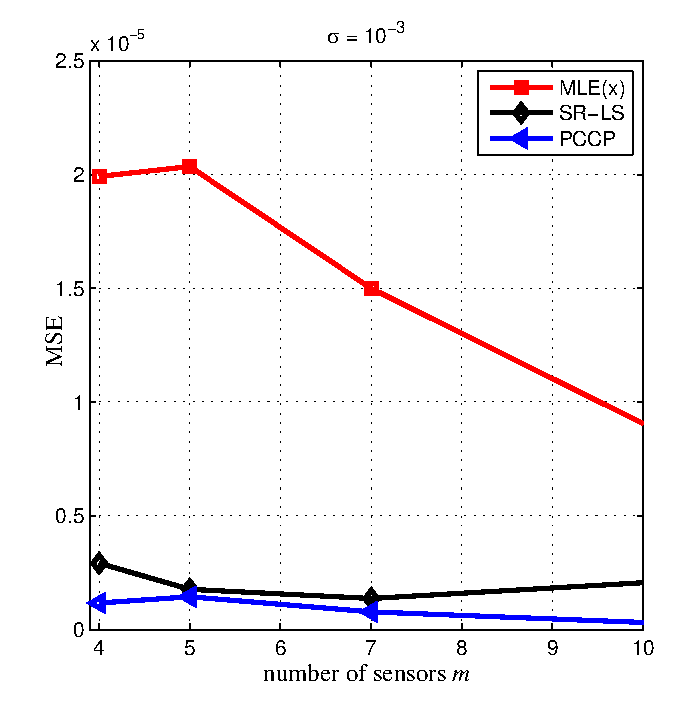
\includegraphics[width=0.5\textwidth,height =0.45\textheight]{figures/ccp/MSE_1e3_sensors}
 &
  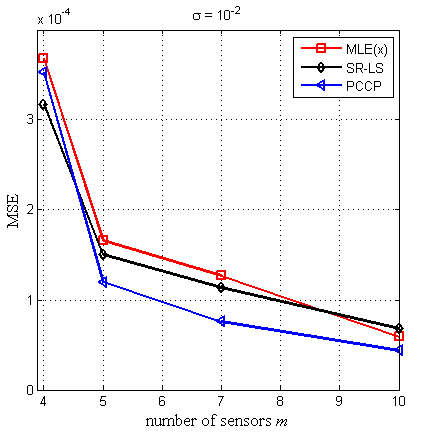
\includegraphics[width=0.5\textwidth,height =0.45\textheight]{figures/ccp/MSE_1e2_sensors} 
  \\   (a)&  (b)   \\
 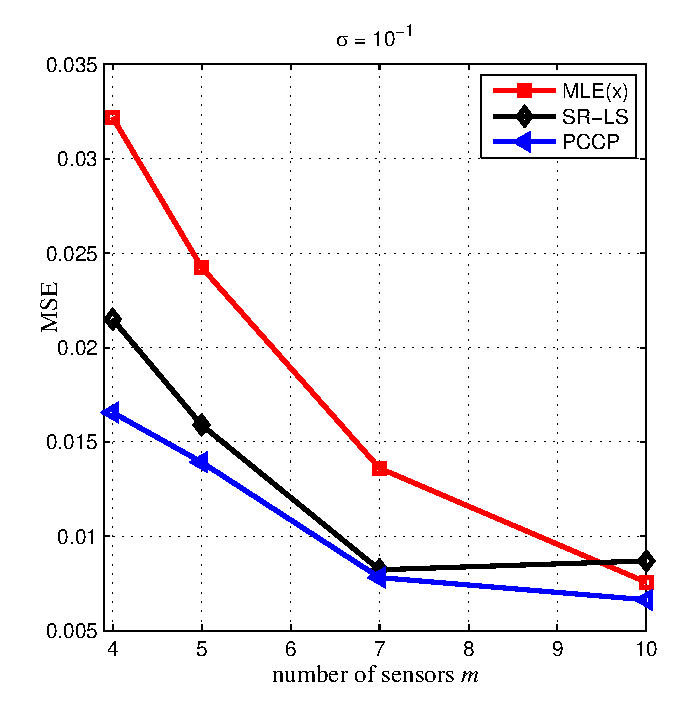
\includegraphics[width=0.5\textwidth,height =0.45\textheight]{figures/ccp/MSE_1e1_sensors}
&
  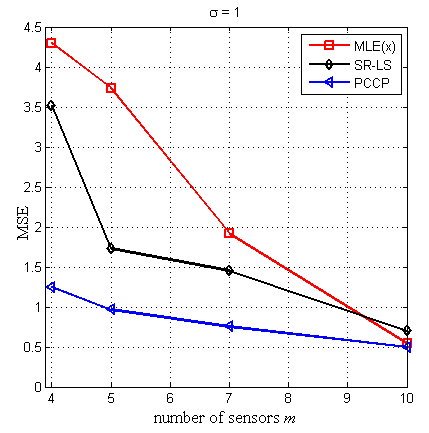
\includegraphics[width=0.5\textwidth,height =0.45\textheight]{figures/ccp/MSE_1e0_sensors} 
    \\  (c)&  (d)   \\
\end{tabular}
\caption{MSE for different methods, various number of sensor nodes $m$ and different noise levels with (a) $\protect\sigma = 10\protect^{-3}$, (b) $\protect\sigma = 10\protect^{-2}$, (c) $\protect\sigma = 10\protect^{-1}$, and (d) $\protect\sigma = 1$.} \label{fig:MSE}
\end{figure}

\begin{figure} 
\centering
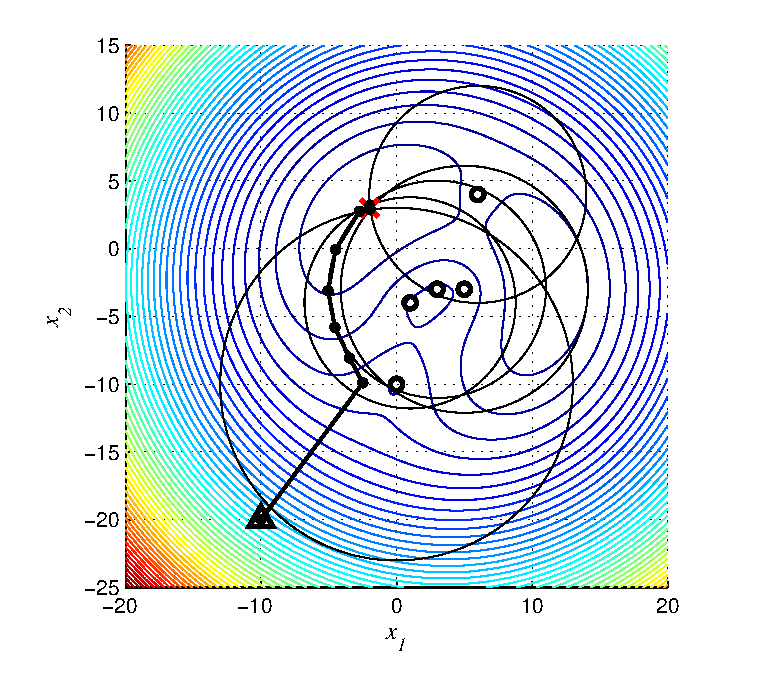
\includegraphics{figures/ccp/iteration_path2}
\caption{Iteration path of the PCCP-based LS Algorithm and contours of the R-LS objective function over the region $\protect\Re = \protect\lbrace \protect\Bx:-15\protect\leq x_1 \protect\leq 15, -25\protect\leq x_2 \protect\leq 15 \protect\rbrace$. The red cross indicates the location of the signal source. Sensors are located at $(6,4)^T$, $(0,-10)^T$, $(5,-3)^T$, $(1,-4)^T$ and  $(3,-3)^T$. Large circles denote possible source locations given the noisy range reading at a particular sensor.}
\label{fig:path}
\end{figure}

\begin{figure}[t] 
\centering
\begin{tabular}{cc}
 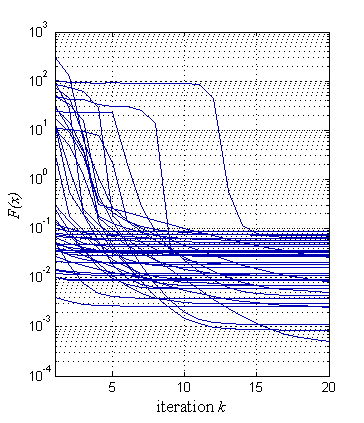
\includegraphics[width=0.5\textwidth,height =0.45\textheight]{figures/ccp/convergence_m4_2}
&
  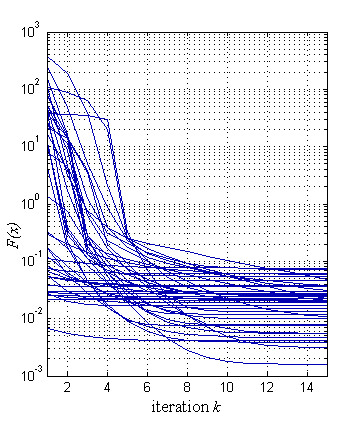
\includegraphics[width=0.5\textwidth,height =0.45\textheight]{figures/ccp/convergence_m5_2_.png} 
  \\   (a) & (b)    \\
 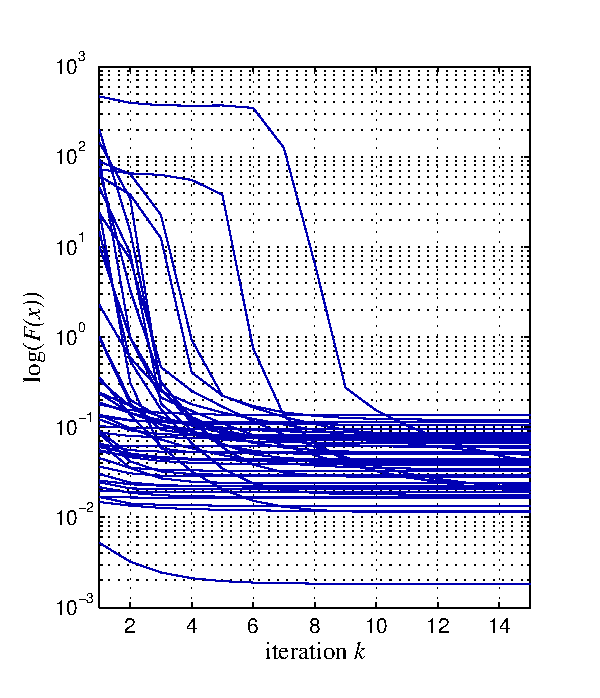
\includegraphics[width=0.5\textwidth,height =0.45\textheight]{figures/ccp/convergence_m7_2}    
 &
  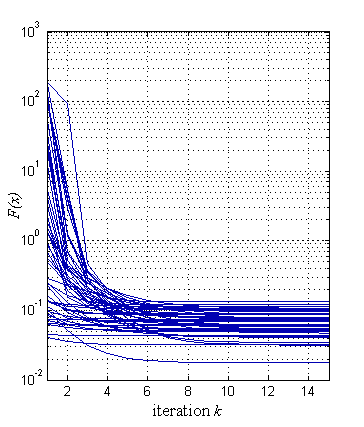
\includegraphics[width=0.5\textwidth,height =0.45\textheight]{figures/ccp/convergence_m10_2_.png} 
  \\   (c) & (d)  
\end{tabular}
\caption{Convergernce of the proposed PCCP-based LS for random initializations with $\protect\sigma = 10\protect^{-1}$ for (a) 4 sensor nodes, (b) 5 sensor nodes, (c) 7 sensor nodes, and (d) 10 sensor nodes.} 
\label{fig:convergence}
\end{figure}